create functions which map inputs to desired outputs by analysing underlying patterns
\begin{itemize}
    \item Regression: find output value $\in \mathbb{R}$ based on input. Example: given a house has 5 bedrooms, 1000 square meters, what is its price?
    \item Classification: assign element to a group. Example: Based on color and texture, is a mushroom edible?
\end{itemize}

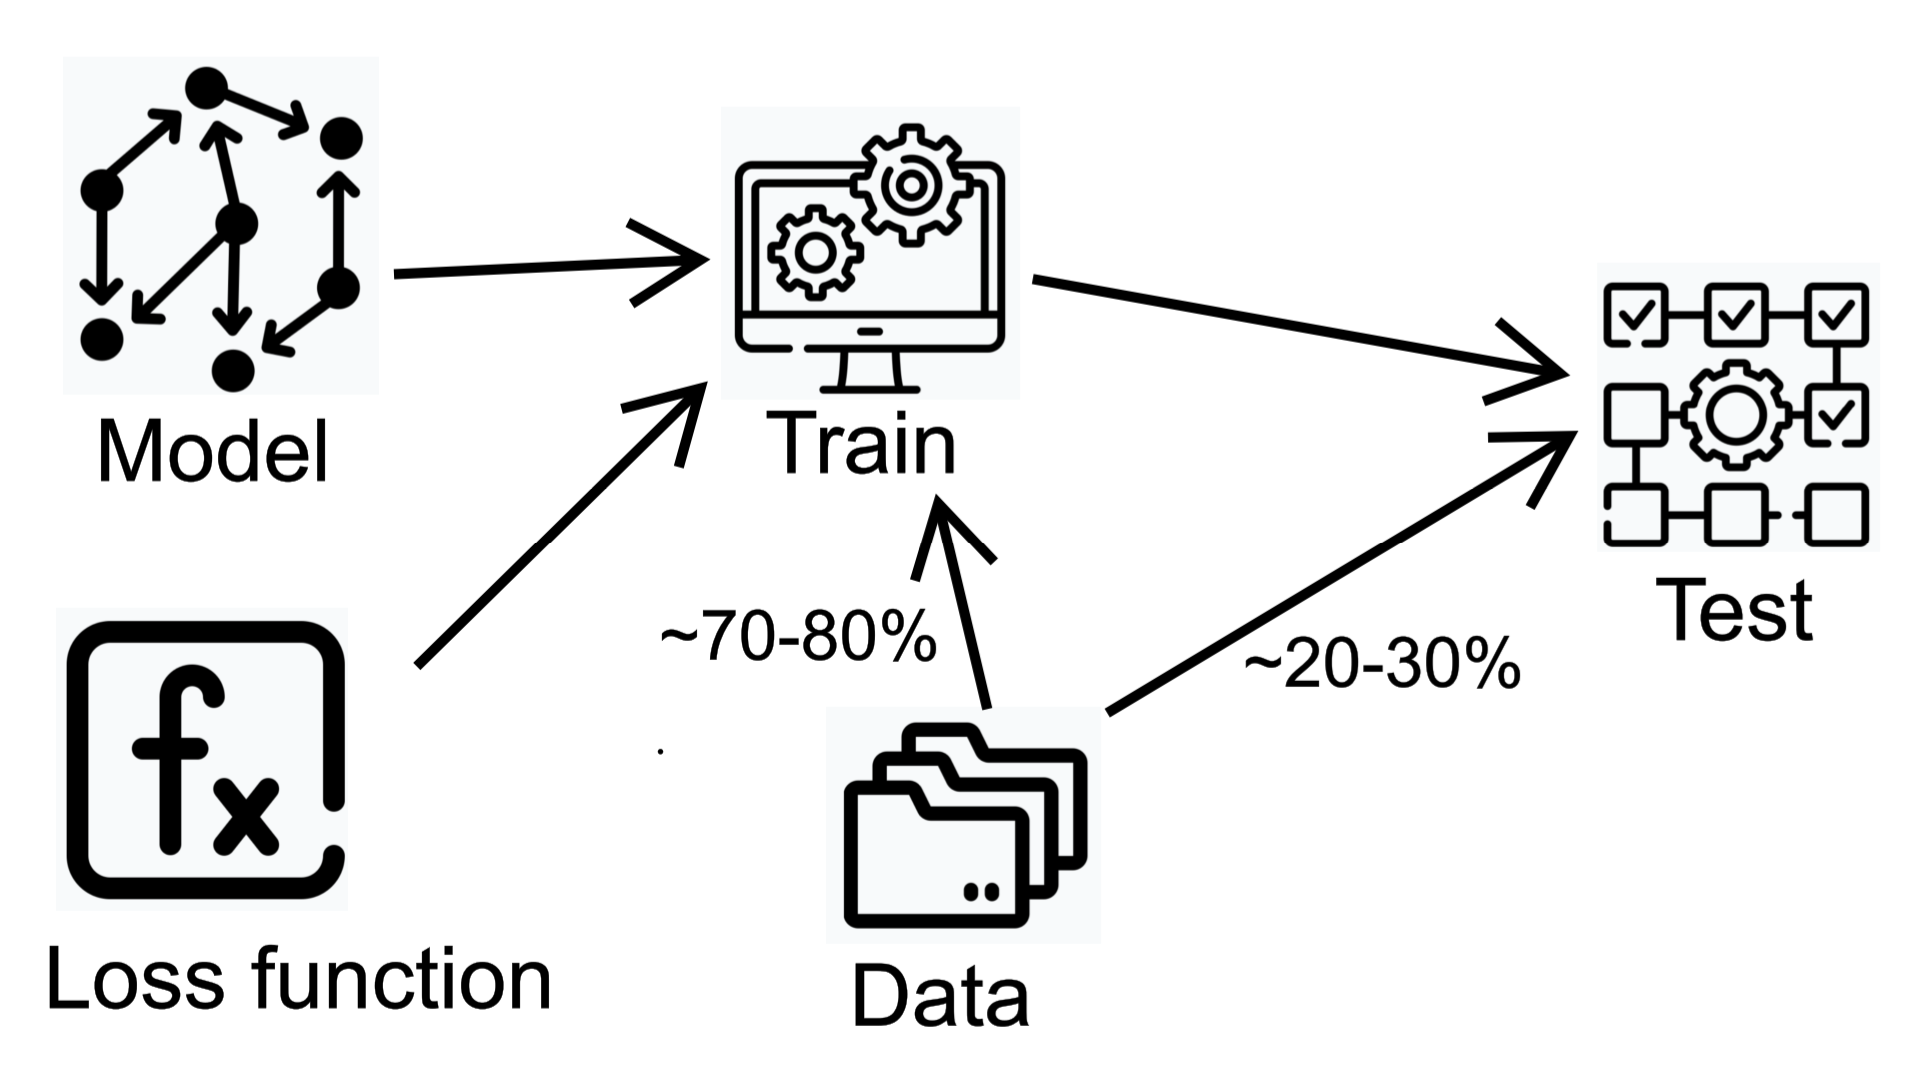
\includegraphics[width = \linewidth]{src/8_ml/images/ml_overview.png}
\lstinputlisting{src/8_ml/code/ml_example.py}

Loss function:
\begin{itemize}
    \item $\frac{\text{\# wrongly classified examples}}{\text{\# total examples}}$
    \item Mean Square Error (MSE)
    \item L2 (Gauss Loss)
\end{itemize}